\documentclass[12pt]{article}
\usepackage[margin=1in]{geometry}
\usepackage{times}
\usepackage{graphicx}
\usepackage{float}
\usepackage{caption}
\usepackage{subcaption}
\author{Danika MacDonell}
\title{Candidacy Report Outline}
\begin{document}
\maketitle

\section{Intro}
\begin{itemize}
\item Briefly introduce the proposed DM search channel
\item Explain what we hope to achieve with the channel: fit to dark higgs candidate mass to search for above-bkg excess
\item If no excess found:
\begin{itemize}
	\item Set limits in m(s), m(Z') phase space
	\item Stat combination with hadronic analysis 
	\item RECAST analysis to enable future re-interpretation of final state with other signal models
\end{itemize}
\end{itemize}
\section{Motivation}
\subsection{Theory}
\begin{itemize}
\item Briefly review evidence for DM from astrophysics
\item Discuss simplified vs. UV complete approaches to DM signal models (ref: 2HDMa whitepaper)
\item Describe why simplified models are useful for mono-X models in particular
\item Introduce the simplified model used for the search (ref: DESY-17-016)
\end{itemize}
\begin{figure}[H]
	\centering
	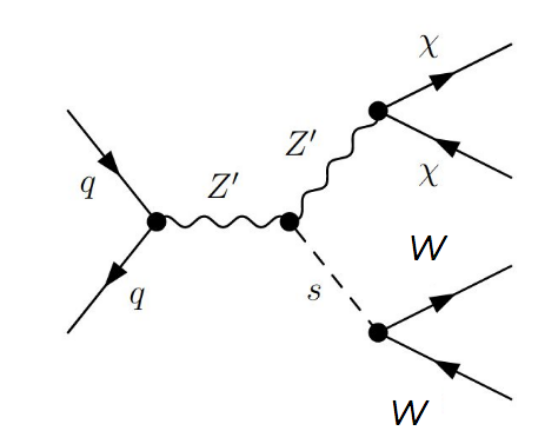
\includegraphics[width=0.4\textwidth]{figures/Signal.png}
	\caption{Signal model}
	\label{fig:signal}
\end{figure}

\subsection{Experimental Background}
\subsubsection{Re-interpretation of mono-H(bb) search for dark higgs mediator}
\begin{figure}[H]
	\centering
	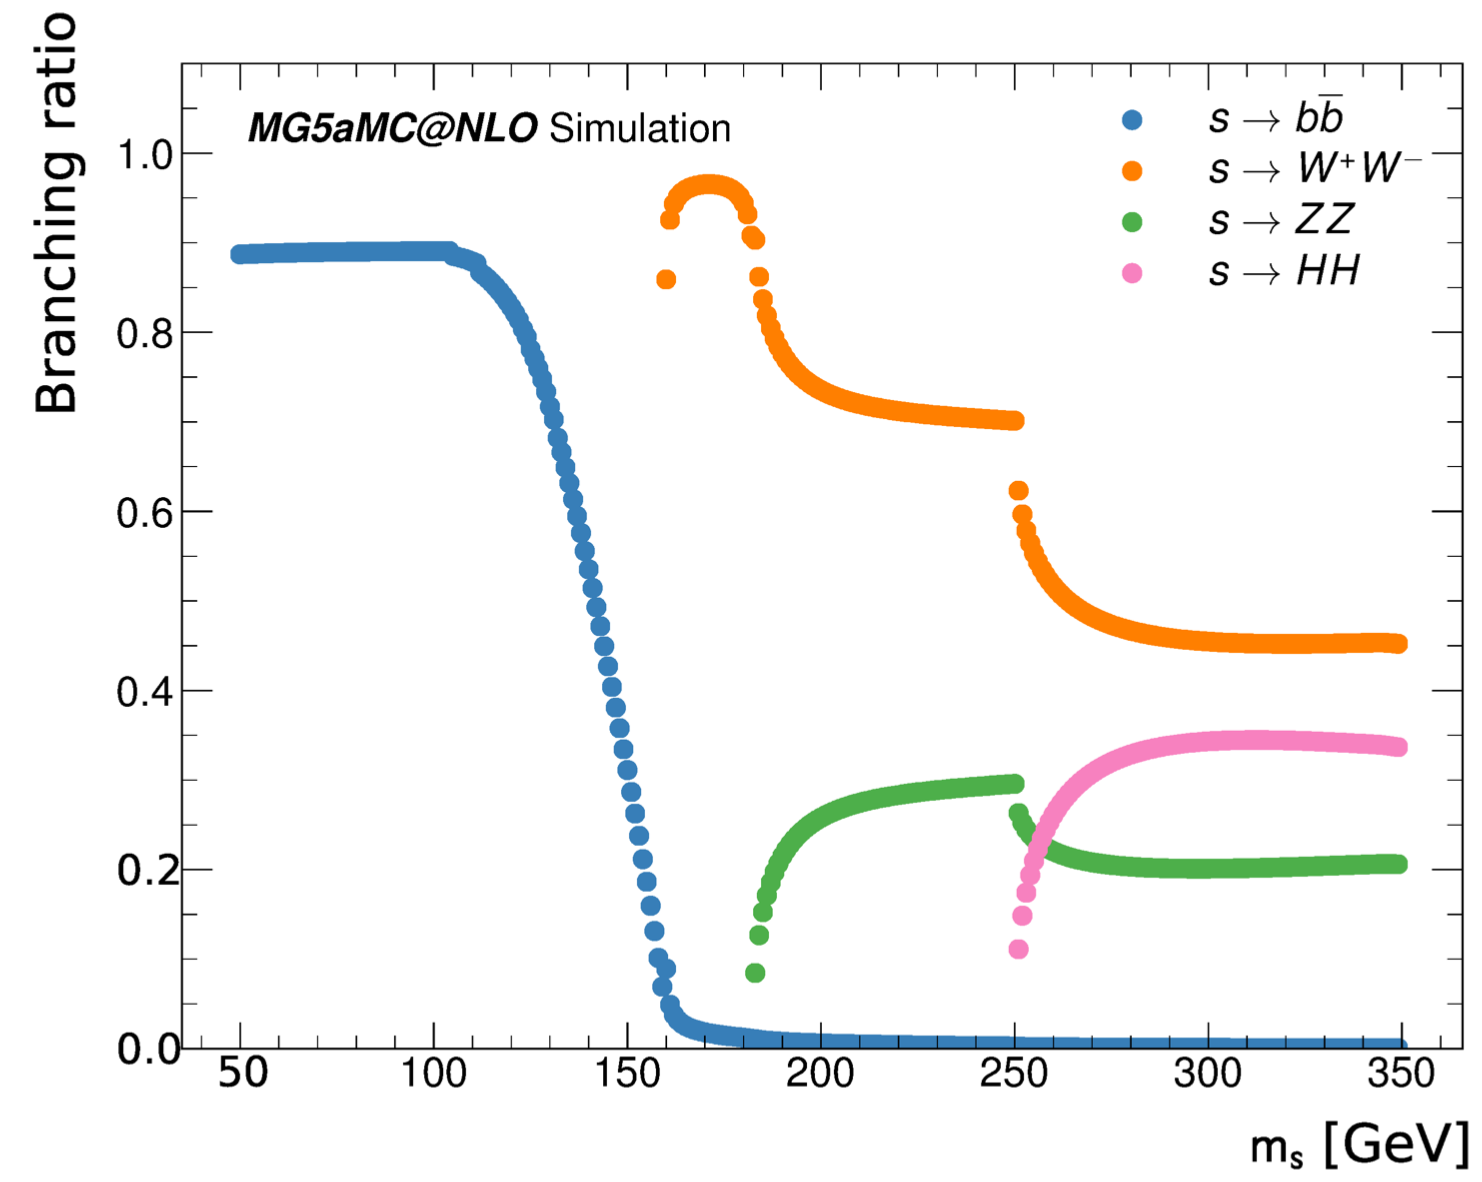
\includegraphics[width=0.7\textwidth]{figures/BR_vs_mass.png}
	\caption{Higgs decay branching ratios as a function of Higgs boson mass}
	\label{fig:higgsbrs}
\end{figure}
\begin{figure}[H]
	\centering
	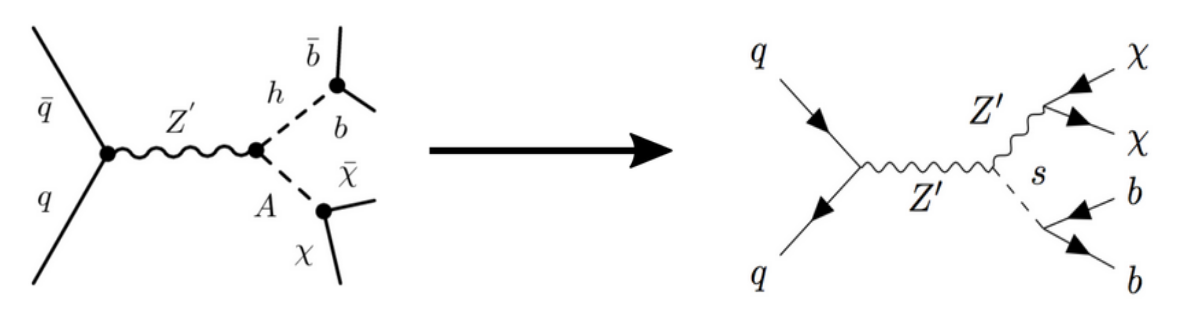
\includegraphics[width=0.9\textwidth]{figures/monohbb_reinterpretation.png}
	\caption{Re-interpretation of mono-H(bb) search using dark higgs boson with floating mass}
	\label{fig:monohbbreinterp}
\end{figure}

\section{Brief intro to LHC and ATLAS detector}
\begin{figure}[H]
	\centering
	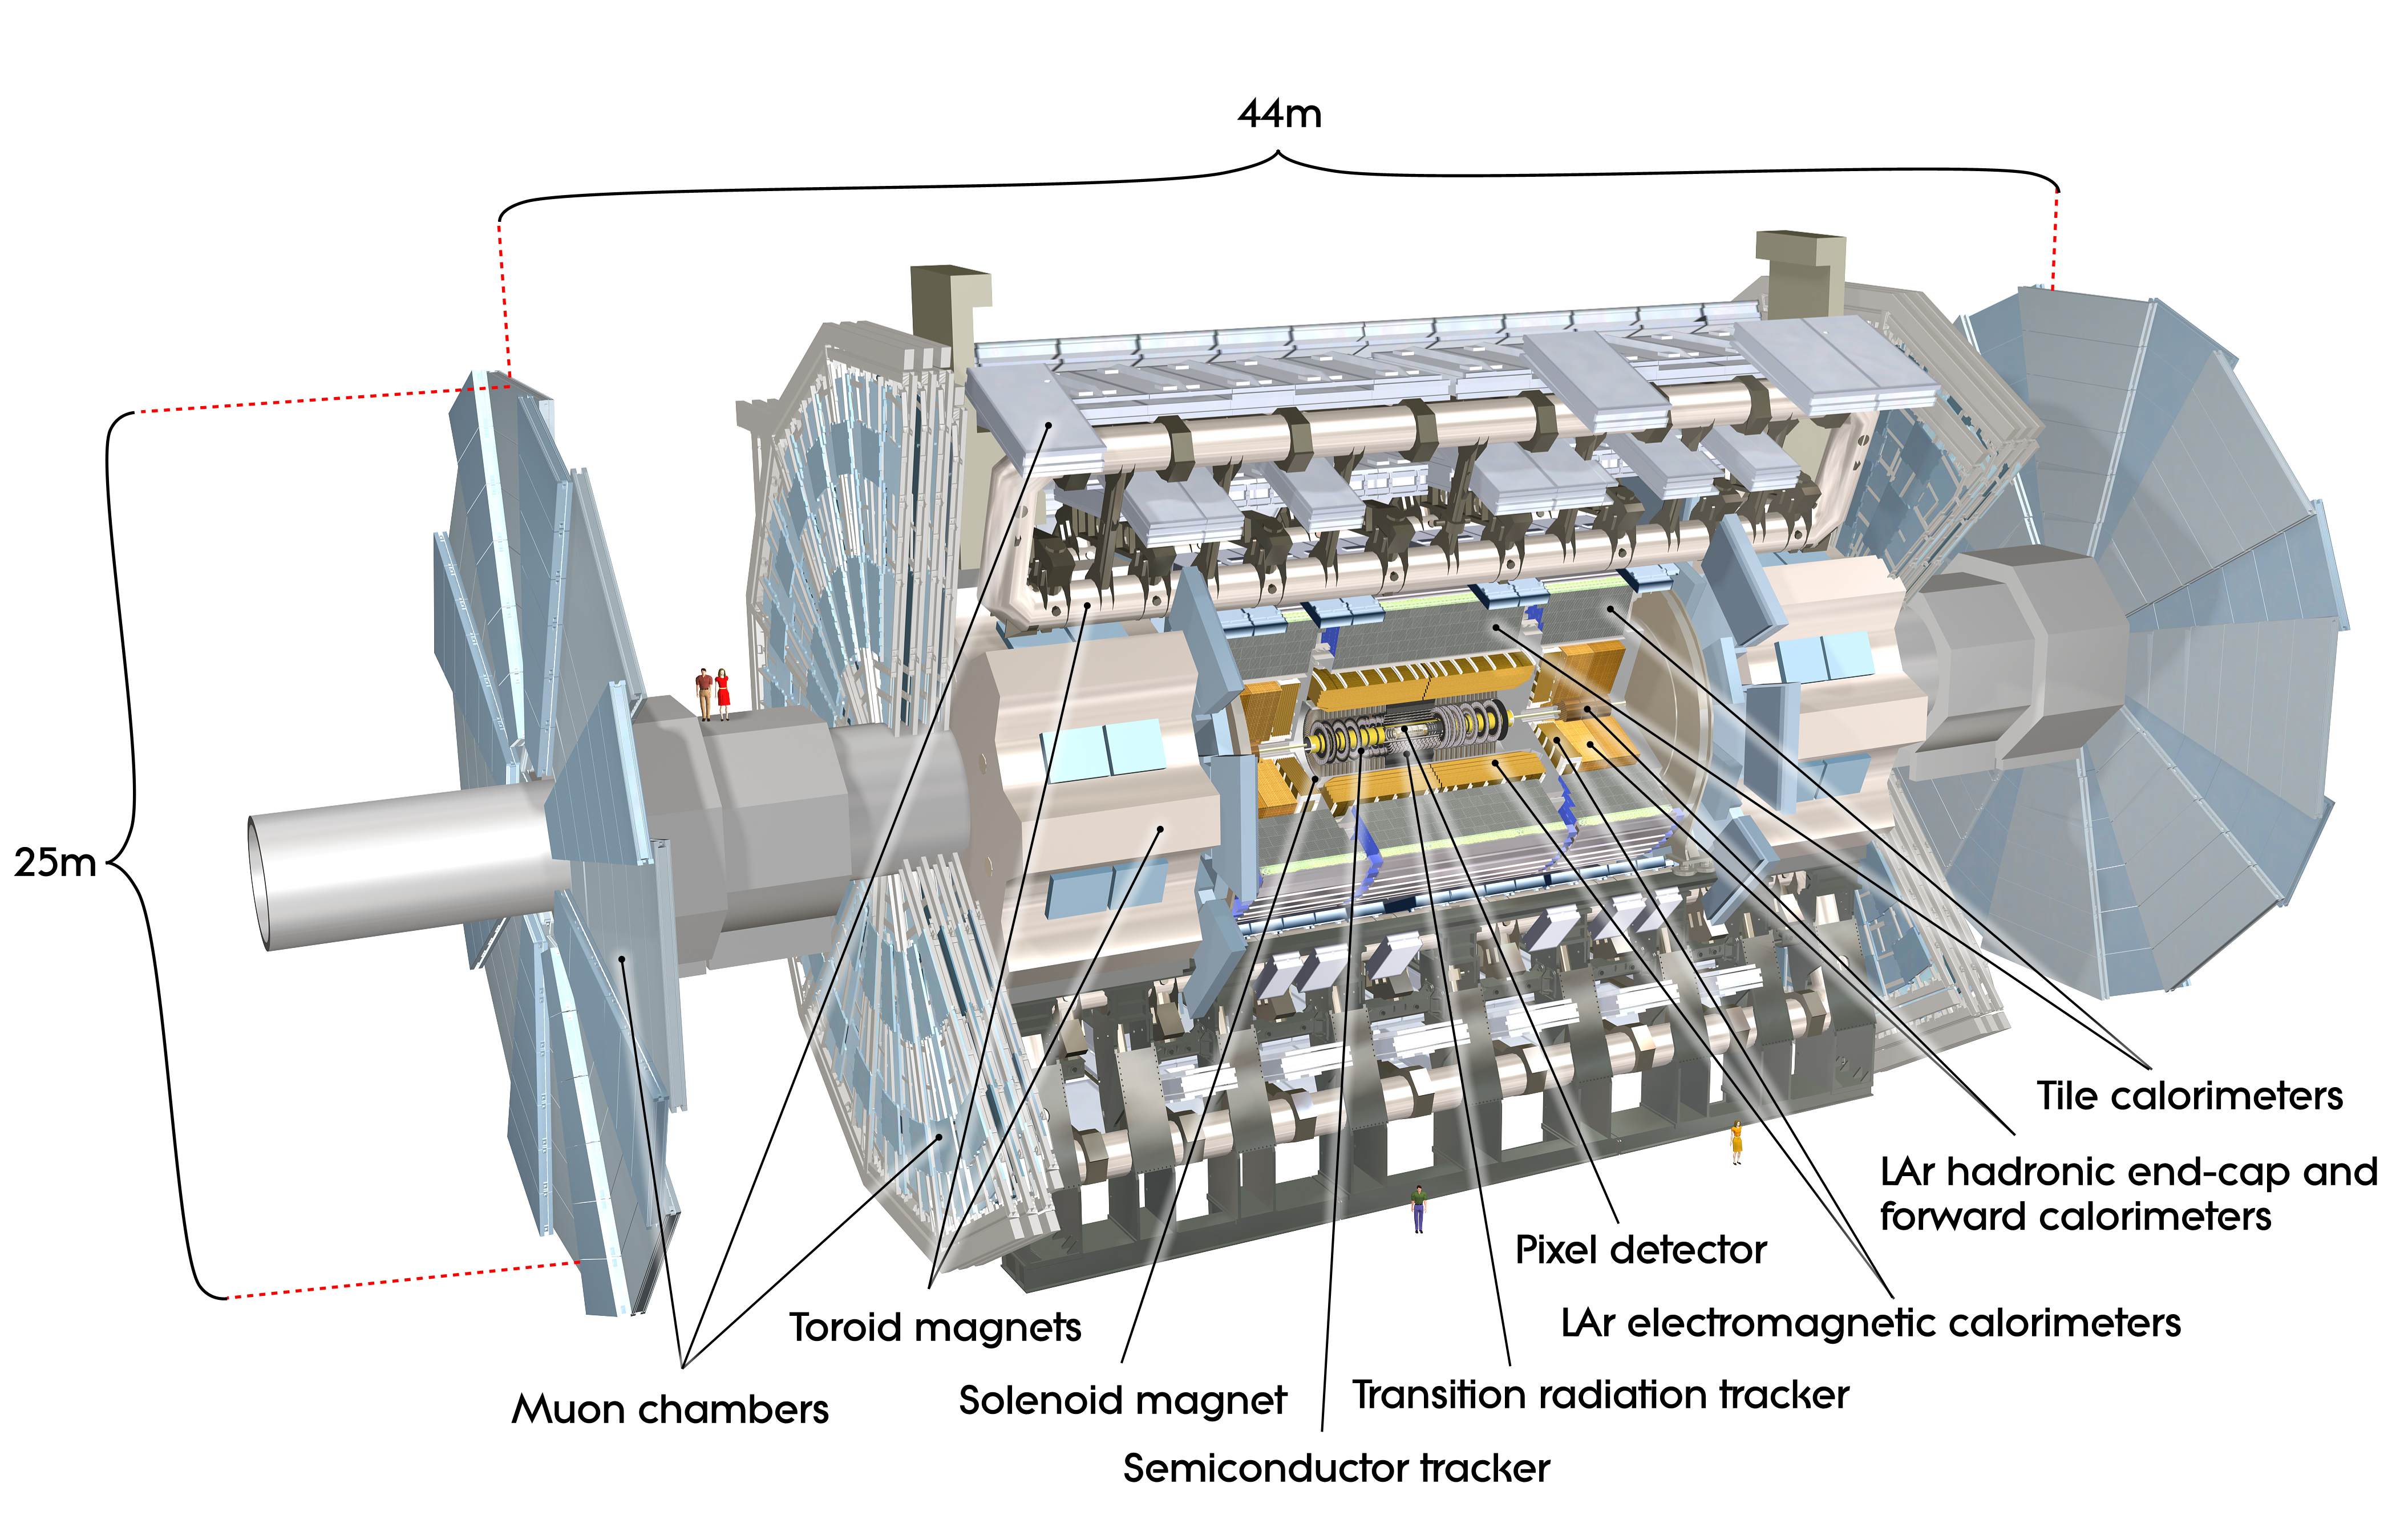
\includegraphics[width=0.85\textwidth]{figures/detector.jpg}
	\caption{ATLAS detector}
	\label{fig:detector}
\end{figure}
\begin{itemize}
\item Inner detector
\item EM cal
\item Had cal
\item Muon spectrometer
\end{itemize}

\section{Ongoing analysis of mono-s(WW) hadronic channel}
\begin{itemize}
\item Preselection
\item Signal region selection
\item Control regions
\item Very brief summary of systematics (exp and modeling)
\item Sensitivity estimates
\item RECAST
\end{itemize}

\section{Signal Sample Generation for Semileptonic Channel}
\begin{figure}[H]
	\centering
	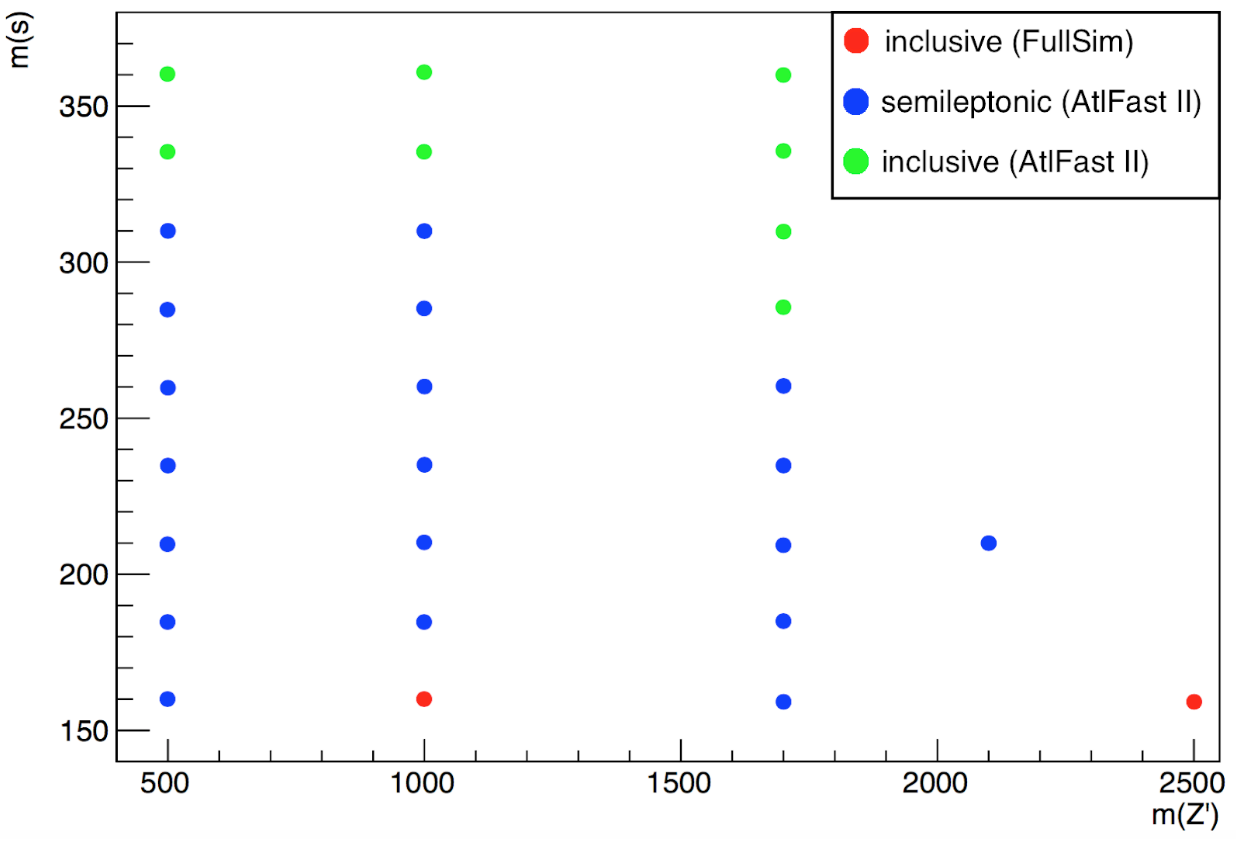
\includegraphics[width=0.7\textwidth]{figures/SignalGrid.png}
	\caption{Grid of signal points with respect to dark higgs (s) and Z' boson masses of generated signal sample}
	\label{fig:signalgrid}
\end{figure}

\begin{itemize}
	\item Scan over range of m(s) and m(Z')
	\item Need to fix some parameters in the model:
	\begin{itemize}
		\item $g_{q} = 0.25$
		\item $g_{\chi} = 1$
		\item $\theta = 0.01$
		\item $m_{\chi} = 200$ GeV
	\end{itemize}
	\item Discuss motivation for above choices of fixed model parameters
\end{itemize}

\section{Event Selection for Semileptonic Channel}

\subsection{Preselection}
\begin{itemize}
\item MET trigger passed
\item 1 signal lepton
\item MET > 150 GeV
\end{itemize}
\subsection{Regions}
\begin{itemize}
\item Signal region
\item W+jets control region
\item ttbar control region (if we plan to do one)
\end{itemize}
\subsection{Categories}
\begin{figure}[H]
     \centering
     \begin{subfigure}[b]{0.4\textwidth}
         \centering
         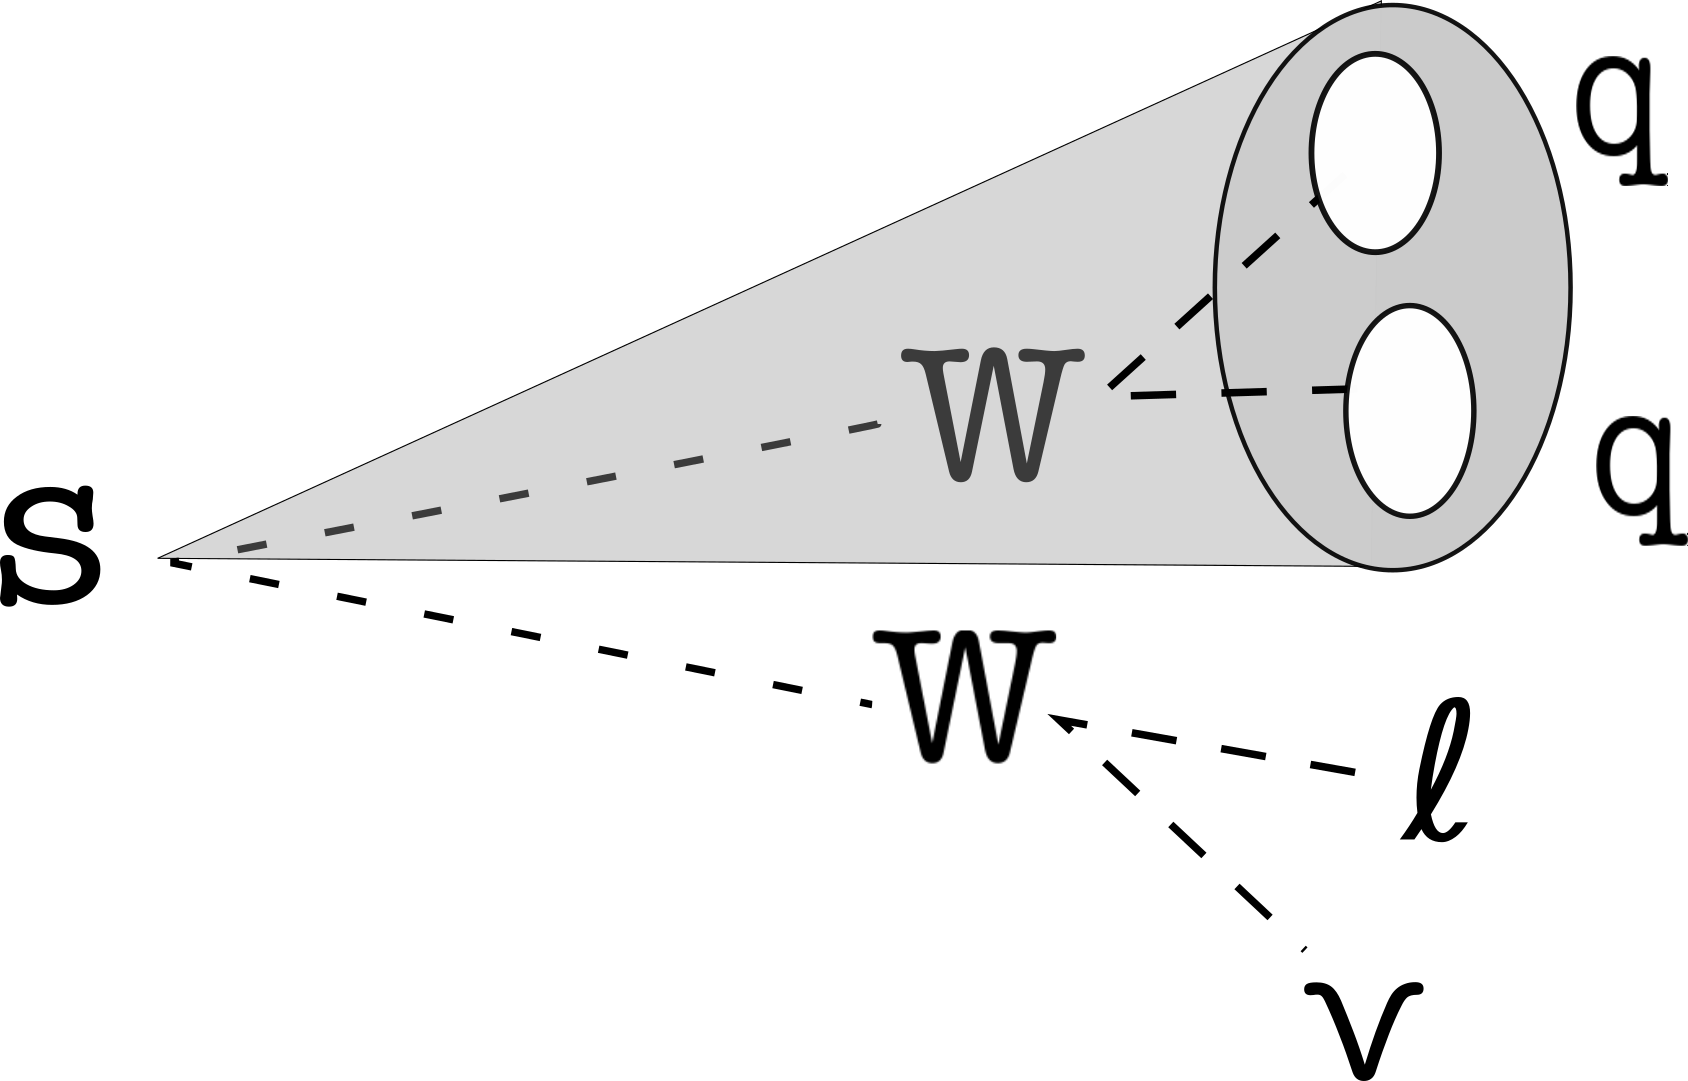
\includegraphics[width=0.9\textwidth]{figures/merged.png}
         \caption{Merged category}
         \label{fig:merged}
     \end{subfigure}
     \hfill
     \begin{subfigure}[b]{0.4\textwidth}
         \centering
         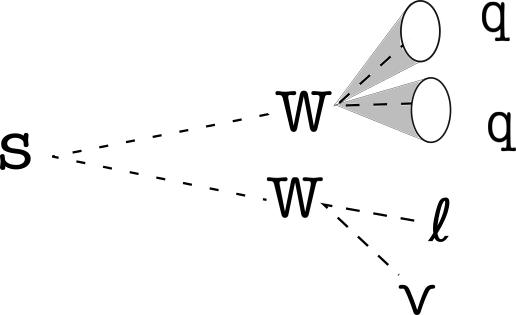
\includegraphics[width=0.9\textwidth]{figures/resolved.png}
         \caption{Resolved category}
         \label{fig:resolved}
     \end{subfigure}
\caption{Kinematic categories for final state selection}
\label{fig:categories}
\end{figure}
\begin{itemize}
\item Resolved category
\item Merged category
\end{itemize}


\section{Sensitivity Studies}
\subsection{Background on limit setting}
\subsection{HistFitter setup}
\begin{itemize}
\item Fit variable
\item Binning
\item Use of temporary systematics proxy
\end{itemize}
\subsection{Preliminary sensitivity limits}
\begin{itemize}
\item Resolved 
\item Merged 
\item Combined
\end{itemize}

\section{Remaining Work and Outlook}
\begin{itemize}
\item Study variables to help address $p_\nu$ vs. $p_{\chi\bar{\chi}}$ MET ambiguity
\item Finalize SR and CR definitions
\item Experimental and modeling systematics
\item Finalize sensitivity estimates with final systematics
\item Statistical combination with hadronic channel for combined limits
\end{itemize}

\end{document}